
\begin{tikzpicture}[
    x = 1.5cm,
    y = 1cm,
    scale=1,
    >=stealth,
    atom/.style = {circle, fill=black, minimum size=8pt,
              inner sep=0pt, outer sep=0pt},
    ]
\clip (-0.5, 0.5) rectangle (2.5, -1.5);
\node () at (0, 0) { 
\begin{tikzpicture}[
    x = 1.2cm,
    y = 0.8cm,
    scale=0.3,
    >=stealth,
    atom/.style = {circle, fill=black, minimum size=5pt,
              inner sep=0pt, outer sep=0pt},
    ]

\node[atom, opacity=0.2] (atom_1) at (0,1){};
\node[atom, opacity=0.2] (atom_2) at (1,0){};
\node[atom, opacity=0.2] (atom_3) at (2,1){};
\node[atom, opacity=0.2] (atom_4) at (3,0){};
\draw [black, solid, very thick, opacity=0.2] (atom_1) -- (atom_2);
\draw [black, solid, very thick, opacity=0.2] (atom_2) -- (atom_3);
\draw [black, solid, very thick, opacity=0.2] (atom_3) -- (atom_4);
\draw [->,black, solid, thick] (atom_2) to node [midway, above]{} (atom_1);
\draw [black, solid, thick] (atom_1) to node [midway, above]{} (atom_2);

\node [atom, fill=black, opacity=1] () at (atom_1){};


\end{tikzpicture}

 };
\node () at (1, 0) { 
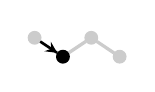
\begin{tikzpicture}[
    x = 1.2cm,
    y = 0.8cm,
    scale=0.3,
    >=stealth,
    atom/.style = {circle, fill=black, minimum size=5pt,
              inner sep=0pt, outer sep=0pt},
    ]

\node[atom, opacity=0.2] (atom_1) at (0,1){};
\node[atom, opacity=0.2] (atom_2) at (1,0){};
\node[atom, opacity=0.2] (atom_3) at (2,1){};
\node[atom, opacity=0.2] (atom_4) at (3,0){};
\draw [black, solid, very thick, opacity=0.2] (atom_1) -- (atom_2);
\draw [black, solid, very thick, opacity=0.2] (atom_2) -- (atom_3);
\draw [black, solid, very thick, opacity=0.2] (atom_3) -- (atom_4);
\draw [->,black, solid, thick] (atom_1) to node [midway, above]{} (atom_2);
\draw [black, solid, thick] (atom_2) to node [midway, above]{} (atom_1);

\node [atom, fill=black, opacity=1] () at (atom_2){};


\end{tikzpicture}

 };
\node () at (2, 0) { 
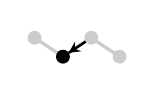
\begin{tikzpicture}[
    x = 1.2cm,
    y = 0.8cm,
    scale=0.3,
    >=stealth,
    atom/.style = {circle, fill=black, minimum size=5pt,
              inner sep=0pt, outer sep=0pt},
    ]

\node[atom, opacity=0.2] (atom_1) at (0,1){};
\node[atom, opacity=0.2] (atom_2) at (1,0){};
\node[atom, opacity=0.2] (atom_3) at (2,1){};
\node[atom, opacity=0.2] (atom_4) at (3,0){};
\draw [black, solid, very thick, opacity=0.2] (atom_1) -- (atom_2);
\draw [black, solid, very thick, opacity=0.2] (atom_2) -- (atom_3);
\draw [black, solid, very thick, opacity=0.2] (atom_3) -- (atom_4);
\draw [->,black, solid, thick] (atom_3) to node [midway, above]{} (atom_2);
\draw [black, solid, thick] (atom_2) to node [midway, above]{} (atom_3);

\node [atom, fill=black, opacity=1] () at (atom_2){};


\end{tikzpicture}

 };

\node () at (0, -1) { 
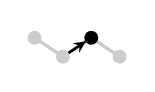
\begin{tikzpicture}[
    x = 1.2cm,
    y = 0.8cm,
    scale=0.3,
    >=stealth,
    atom/.style = {circle, fill=black, minimum size=5pt,
              inner sep=0pt, outer sep=0pt},
    ]

\node[atom, opacity=0.2] (atom_1) at (0,1){};
\node[atom, opacity=0.2] (atom_2) at (1,0){};
\node[atom, opacity=0.2] (atom_3) at (2,1){};
\node[atom, opacity=0.2] (atom_4) at (3,0){};
\draw [black, solid, very thick, opacity=0.2] (atom_1) -- (atom_2);
\draw [black, solid, very thick, opacity=0.2] (atom_2) -- (atom_3);
\draw [black, solid, very thick, opacity=0.2] (atom_3) -- (atom_4);
\draw [->,black, solid, thick] (atom_2) to node [midway, above]{} (atom_3);
\draw [black, solid, thick] (atom_3) to node [midway, above]{} (atom_2);

\node [atom, fill=black, opacity=1] () at (atom_3){};


\end{tikzpicture}

 };
\node () at (1, -1) { 
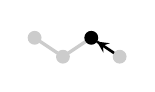
\begin{tikzpicture}[
    x = 1.2cm,
    y = 0.8cm,
    scale=0.3,
    >=stealth,
    atom/.style = {circle, fill=black, minimum size=5pt,
              inner sep=0pt, outer sep=0pt},
    ]

\node[atom, opacity=0.2] (atom_1) at (0,1){};
\node[atom, opacity=0.2] (atom_2) at (1,0){};
\node[atom, opacity=0.2] (atom_3) at (2,1){};
\node[atom, opacity=0.2] (atom_4) at (3,0){};
\draw [black, solid, very thick, opacity=0.2] (atom_1) -- (atom_2);
\draw [black, solid, very thick, opacity=0.2] (atom_2) -- (atom_3);
\draw [black, solid, very thick, opacity=0.2] (atom_3) -- (atom_4);
\draw [->,black, solid, thick] (atom_4) to node [midway, above]{} (atom_3);
\draw [black, solid, thick] (atom_3) to node [midway, above]{} (atom_4);

\node [atom, fill=black, opacity=1] () at (atom_3){};


\end{tikzpicture}

 };
\node () at (2, -1) { 
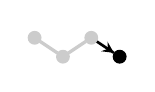
\begin{tikzpicture}[
    x = 1.2cm,
    y = 0.8cm,
    scale=0.3,
    >=stealth,
    atom/.style = {circle, fill=black, minimum size=5pt,
              inner sep=0pt, outer sep=0pt},
    ]

\node[atom, opacity=0.2] (atom_1) at (0,1){};
\node[atom, opacity=0.2] (atom_2) at (1,0){};
\node[atom, opacity=0.2] (atom_3) at (2,1){};
\node[atom, opacity=0.2] (atom_4) at (3,0){};
\draw [black, solid, very thick, opacity=0.2] (atom_1) -- (atom_2);
\draw [black, solid, very thick, opacity=0.2] (atom_2) -- (atom_3);
\draw [black, solid, very thick, opacity=0.2] (atom_3) -- (atom_4);
\draw [->,black, solid, thick] (atom_3) to node [midway, above]{} (atom_4);
\draw [black, solid, thick] (atom_4) to node [midway, above]{} (atom_3);

\node [atom, fill=black, opacity=1] () at (atom_4){};


\end{tikzpicture}

 };


\end{tikzpicture}
